\section{Introduction}
A carbon calculation error can increase the total value of a green investment portfolio while reducing the value of investments that meet its environmental mandate. We show how errors in carbon intensity, the emissions generated per unit of electricity, create this outcome. We also derive the exact condition under which financing an ineligible project displaces qualifying investment value. We measure financial value using net present value (NPV): the present value of future cash flows minus the initial investment cost.

Consider one of eight constructed portfolios. Dividing emissions by all electricity generated instead of the electricity delivered to the grid makes a USD 40 million project appear eligible. With USD 87.75 million available, financing that project displaces two qualifying investments worth USD 4.40 million in NPV. With USD 117 million available, the lender can fund it alongside the qualifying investments. The same calculation error leads to different financial outcomes because the available capital determines which investments can be retained.

Two public records illustrate the importance of connecting the emissions calculation to the funding decision. At Chile's Copiulemu landfill gas project, a verifier traced an error in the December 2006 methane calculation to a spreadsheet that summed column O instead of column N \citep[p.~11]{sgs}. At Vasilikos Unit~6 in Cyprus, the European Investment Bank estimated emissions of about 380 grams of carbon dioxide per kilowatt-hour on natural gas. This met the ceiling of 550 for projects already under appraisal and exceeded the new ceiling of 250 \citep{eibscore,eibmid}. The bank signed a EUR~76 million loan on 17 December 2020 \citep{eibloan}. The Chilean record establishes a calculation error; the Cypriot record documents financing under an emissions policy. Valuing displaced opportunities also requires the competing projects, their financial inputs and the applicable budget.

Carbon accounting provides the emissions information that organizations use to implement environmental strategy. Drawing on qualitative responses from 44 industry experts, \citet{ruan2026} describe the governance arrangements, capabilities and infrastructure that embed carbon accounting in organizations. \citet{wu2026} examine implementation barriers and strategies through a mixed-method study incorporating 53 studies and industry-expert responses. For a lender that applies an emissions ceiling, the calculation has a direct role in implementing strategy: it determines which investments can compete for capital.

The financial consequence matters for clean energy finance, including the investment in technology and infrastructure called for in Target~7.a of Sustainable Development Goal~7 \citep{un}. Funding records can establish how much money was committed to projects outside the mandate. To assess the opportunity cost, an investment committee must also determine which qualifying investments could have been funded with that money. This requires comparing the reported allocation with the best alternatives available under the approved rule.

Checking the rule begins with identifying the calculation that the software actually performs. A key performance indicator (KPI) is a measure used to assess performance; in this study, the indicator is carbon intensity. Literate programming presents executable code together with an explanation of what it does \citep{knuth}. LEAP (Literate Programming for Automated KPI Extraction) is a research engine that applies this approach to KPI documentation. It recovers written formulas and links them to the relevant code \citep{zenodo,leap}. We use those links to identify the stated emissions formula and its implementation in each program, then check the calculated values against the approved rule.

Our objective is to establish what an eligibility error costs when projects compete for a fixed capital budget. We compare funding under the approved formula with funding under three altered calculations. The analysis separates the value lost when qualifying projects are excluded from the value displaced when ineligible projects receive funding. It establishes when displacement begins, how the losses vary with the budget and emissions ceiling, and how many eligibility checks can determine the funded portfolio when the formula is uncertain. These results connect the accuracy of carbon accounting to the financial execution of an environmental investment strategy.

\section{From carbon measurement to investment choice}
Green finance directs investment toward environmental objectives. In their review of green and climate finance, \citet{joshipura2025} identify transition finance, eco-innovation, funding sources and enabling conditions as related research themes. From the perspective of lenders, \citet{raimondi2026} synthesize research on incorporating climate considerations into bank credit-risk assessment. These studies situate environmental information within financial decisions. Our focus is the rule a lender uses to determine which projects qualify for green financing.

\subsection{Measurement choices and investment eligibility}
The financial consequences of environmental measurement begin with the way an indicator is defined. \citet{berg} explain why environmental, social and governance (ESG) ratings can differ for the same company: providers measure different attributes, use different measurement procedures and assign different weights. \citet{lohmann} examine a consequence for investors: requiring agreement among ratings providers can narrow the set of investments they are permitted to hold. The accountability framework developed by \citet{tian2026} traces such disagreement through the measurement process across jurisdictions. At the level of carbon accounting, \citet{anquetin} compare two emissions datasets and examine how including emissions from a company's value chain affects green equity portfolios. Together, this research shows how measurement choices shape investment selection.

Investment eligibility can also change when data or calculations depart from their intended meaning. \citet{gurvich2021} document how multiple security listings and index construction can attribute too much carbon to a company. They explain how distorted data can cause unjustified exclusions or reductions in portfolio weights. \citet{bajic2023} identify inconsistencies in company-level emissions data, including mismatched reporting periods, and show that changing the intensity denominator can alter company rankings. These findings establish the importance of carbon-data accuracy for investment screening. For a lender operating under an approved emissions rule, they lead to a further question: how much qualifying investment value is lost when an erroneous calculation changes the set of eligible projects?

\subsection{From eligibility errors to financial loss}
The financial consequence of an eligibility error depends on the investments competing for capital. Capital rationing describes the problem of allocating a limited budget among investment opportunities \citep{lorie}. When projects must be funded in full, financing one can prevent another from receiving the required capital. \citet{he} examine this problem for building retrofits by evaluating affordable combinations of projects according to financial returns and energy or emissions benefits. \citet{schoenmaker} examine investment rules that assign explicit weights to financial, environmental and social value. In the decision studied here, the emissions ceiling determines eligibility, and NPV determines the best affordable combination of eligible projects. We define \emph{qualified NPV} as the combined NPV of funded projects that meet the ceiling under the approved formula. This measure allows us to compare the financial value delivered under the mandate with the value the same budget could have delivered under the correct calculation.

Research on the stability of investment choices provides a mathematical foundation for this comparison. \citet{hien} examine how a margin for uncertainty changes the allocations permitted by a risk budget. \citet{pisinger} determine how far an item's value or weight can change while an optimal selection remains optimal. Their analysis uses the lightest value-maximizing combination to leave the greatest unused capacity. In green capital budgeting, the corresponding quantity is the money left after reserving the least expensive portfolio that achieves the highest NPV. Applying this principle to environmental eligibility errors allows us to determine when funding a falsely admitted project displaces qualifying investment value. The remaining loss arises when the erroneous calculation excludes qualifying projects from consideration. Our analysis values these mechanisms separately.

\subsection{From carbon accounting assurance to funding verification}
Sustainability assurance concerns the reliability of the environmental information organizations report and use. Using panel regressions on 6,140 firm-year observations across 39 countries, \citet{ibrahim2026} associate higher sustainability audit quality with lower reported carbon-emission intensity. To connect assurance to the investment decision itself, a reviewer needs to identify whether the implemented calculation follows the approved rule and whether correcting the error changes the funded portfolio.

Evidence of compliance begins with a rule that specifies what to measure. Research on green bonds, which finance activities with environmental objectives, examines the information needed to assess environmental monitoring disclosures \citep{nicolici} and distinguishes alignment with a financing framework from formal certification \citep{loiola}. Once a rule specifies a formula and its inputs, the reviewer can compare the software's calculation with the expected result. The source-linked KPI review method described by \citet{review} illustrates this distinction with gross margin, the share of revenue left after deducting costs. For revenue of 100 and cost of 60, the written formula gives 40\%, whereas the program returns 166.67\%. The same distinction between the stated formula and its implementation provides the basis for verifying emissions calculations.

Determining an optimal investment decision also requires deciding which uncertain inputs must be checked. \citet{schloter} study which uncertain item values need verification to identify an optimal selection. \citet{dughmi} study checks of item availability to obtain a near-optimal expected return. In our setting, project costs and cash flows are known, and each check reveals whether a project meets the emissions ceiling. The reviewer can stop when every possible eligibility pattern consistent with the answers leads to the same funded portfolio. This makes verification part of the capital allocation problem: the aim is to establish the funded portfolio and assess the financial consequences of eligibility errors under the approved rule.

\section{Materials and methods}
Our main research question is: when an erroneous carbon calculation changes project eligibility, how much qualified NPV is lost through exclusion or displacement, and when does displacement begin? We also ask how many eligibility checks are needed to determine the funded portfolio when the formula is uncertain. The research design follows the lender's decision in two stages. First, the emissions ceiling determines which projects qualify. Second, the lender selects the affordable combination of qualifying projects with the highest NPV. We compared funding under the approved formula with funding under three altered calculations, holding the projects, cash flows and budgets fixed. This design isolates the financial consequences of the calculation errors within the constructed portfolios.

\subsection{Project inputs and carbon eligibility}
We constructed eight portfolios of six energy projects each. Projects are indivisible: the lender either funds a project in full or leaves it unfunded. For project $i$, gross generation $G_i$ is the electricity produced, and net exports $Q_i$ are the electricity delivered to the grid. Both are measured in megawatt-hours, with $G_i>Q_i>0$. Scope~1 emissions $S_{1i}$ come directly from the project's operations; Scope~2 emissions $S_{2i}$ arise from producing the energy the project purchases. Both quantities are measured in kilograms of carbon dioxide equivalent (kg CO$_2$e), a common unit that expresses the warming effect of greenhouse gases relative to carbon dioxide, following the Greenhouse Gas Protocol \citep{ghg}. The reference intensity $E_i=(S_{1i}+S_{2i})/Q_i$ measures operating emissions per megawatt-hour (MWh) of electricity exported, excluding emissions over the full project lifecycle and emissions avoided relative to an alternative source of electricity. A project qualifies when its calculated intensity is at or below the ceiling $\tau$.

The 48 project records include intensities near each study ceiling. Starting with six base intensities of 330, 378, 392, 407, 429 and 465~\unit, we adjusted them by portfolio and project position to place projects on either side of the three ceilings of 380, 400 and 420~\unit. Within each portfolio, capital cost and reference intensity both increase with project position. A higher-intensity project admitted by an altered calculation can therefore compete for a substantial share of the budget. Supplement~S1 gives the generator equations, project identifiers and raw inputs.

We used four programs to compare the approved formula with three implementation errors. Each program received the same project inputs and declared the same formula. The reference program returned $E_i$. Using gross generation as the denominator gives $(S_{1i}+S_{2i})/G_i$ and lowers intensity because gross generation exceeds net exports by 7\% to 17\%. Omitting Scope~2 gives $S_{1i}/Q_i$ and lowers intensity because Scope~2 accounts for 9\% to 19\% of total emissions. Both percentages vary with the same combination of portfolio and project indices, the identifiers used to generate the input values. The third alteration understates net exports, giving $(S_{1i}+S_{2i})/(0.85 Q_i)$ and raising intensity by a factor of $1/0.85$. In each primary comparison, all six projects in a portfolio use the same program.

\subsection{Capital budget and financial outcomes}
The financier ranks affordable project combinations by their combined NPV. Each project requires a positive initial outlay $K_i$ and generates five equal end-of-year net cash flows $C_i$. We assign no additional value after year five. The annual discount rate $r_i$, between 7\% and 10\%, converts future cash flows to present value. The resulting NPV in modeled USD millions is $v_i=-K_i+\sum_{t=1}^{5} C_i/(1+r_i)^t$. The financier can spend $b$, set at 45\%, 60\% or 75\% of the capital needed for all six projects. Given the eligible set $A$, the best attainable NPV is
\begin{equation}
\begin{aligned}
 V(A,b)&=\max_{\substack{S\subseteq A\\ K(S)\le b}}v(S),\\
 K(S)&=\sum_{i\in S}K_i,\quad v(S)=\sum_{i\in S}v_i .
 \end{aligned}\label{eq:opt}
\end{equation}
where $K(S)$ and $v(S)$ are the total cost and NPV of a subset $S$. Write $S(A,b)$ for the chosen subset. The financier may leave part or all of the budget unspent, so the empty set is among the 64 possible subsets. Among equally valuable choices the program selects the least expensive. If costs also tie, a fixed subset ordering selects the first maximizer in that ordering. An independent calculation found a unique highest-value subset in every main and control decision.

Let $T$ be the projects that qualify under the approved formula, $R$ the projects that qualify under the reported calculation, and $\widehat S=S(R,b)$ the funded set. Total NPV includes every funded project (termed \emph{nominal NPV} in the supplement). Qualified NPV includes only the funded projects that meet the approved rule, $\widehat S\cap T$. The qualified NPV shortfall measures the value forgone. It is the best attainable NPV under the approved rule minus the qualified NPV of the selected portfolio:
\begin{equation}
 L=V(T,b)-v(\widehat S\cap T). \label{eq:loss}
\end{equation}
We also measure capital committed to ineligible projects as $K(I)$, where $I=\widehat S\setminus T$ contains the falsely admitted projects that received funding. These projects can still generate cash flows even though the mandate credits them with no qualified NPV.

\subsection{Value lost through exclusion and capital displacement}
The loss has two sources. Let $C=T\cap R$ contain the projects that pass both screens. Comparing $T$ with $C$ at the full budget measures the loss from false exclusions: qualifying projects rejected by the erroneous calculation. Keeping $C$ fixed and deducting the capital $K(I)$ spent on false admissions (ineligible projects admitted by the erroneous calculation) measures displacement. The two losses sum to the qualified NPV shortfall,
\begin{equation}
\begin{aligned}
L={}&\underbrace{V(T,b)-V(C,b)}_{\substack{\text{value removed by}\\\text{false exclusions}}}\\
&+\underbrace{V(C,b)-V(C,b-K(I))}_{\substack{\text{qualified value displaced}\\\text{by false admissions}}} .
\end{aligned}
\label{eq:decompose}
\end{equation}
To see why, hold the funded ineligible projects $I$ fixed. The qualified portion of $\widehat S$ must maximize NPV over $C$ at the remaining budget $b-K(I)$ (the residual budget). A more valuable affordable subset of $C$ could be funded alongside $I$ and would improve on the reported optimum. Substituting that residual-budget optimum into Equation~\eqref{eq:loss} gives Equation~\eqref{eq:decompose}.

Each component is nonnegative because removing projects or reducing the budget can only restrict the choice. If the altered screen only admits extra projects, displacement accounts for the entire loss. If it only excludes projects, exclusion accounts for the entire loss. For a mixed error we measure exclusions with all capital available before measuring displacement among the projects still eligible. This accounting assumes additive project costs and NPVs and allows capital to remain unspent.

The displacement threshold is the capital left after reserving the least expensive combination of projects in $C$ that achieves the maximum NPV at budget $b$. Write $c^*(C,b)$ for its cost and $h=b-c^*(C,b)$ for the capital left. Then
\begin{equation}
\begin{gathered}
 V(C,b)-V(C,b-K(I))>0\\
 \Longleftrightarrow\quad K(I)>h .
 \end{gathered}\label{eq:slack}
\end{equation}
If $K(I)\leq h$, at least one value-maximizing portfolio drawn from $C$ remains affordable. If $K(I)>h$, every subset attaining the original value costs more than the residual budget. With finitely many subsets, the best attainable value must then fall. Choosing the least expensive of the tied portfolios therefore gives the threshold even when several portfolios have the same NPV. Figure~\ref{fig:mechanism} connects the two funding decisions to the loss decomposition and the displacement threshold.
\ifdefined\readingcopy\begin{figure*}[!t]
\centering
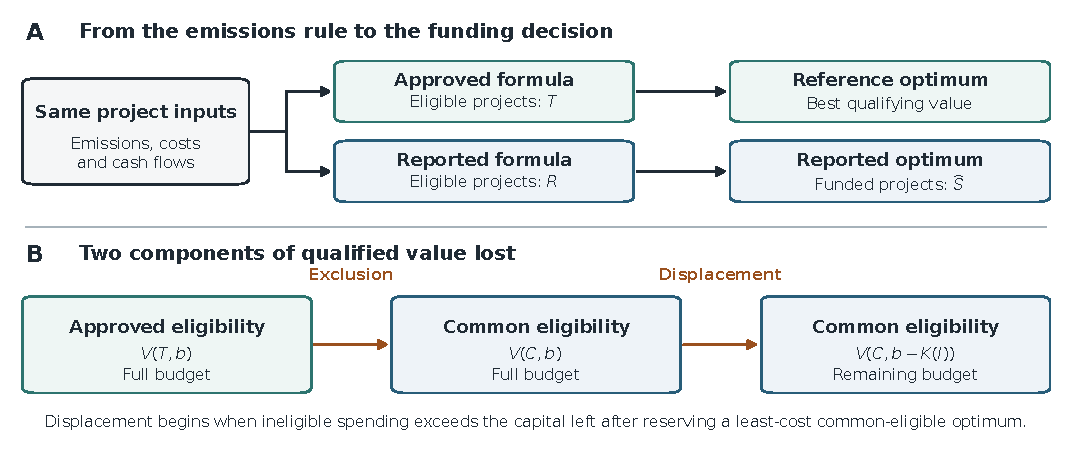
\includegraphics[width=\linewidth]{figures/loss_mechanism.pdf}
\caption{Carbon calculation and qualified investment loss. (A) The approved and reported formulas are applied to identical project inputs and the same budget $b$ and emissions ceiling; $T$ and $R$ denote the respective eligible sets, and $\widehat S$ is the funded set under the reported formula. (B) The successive optimal net present values $V$ separate the loss from removing projects excluded in error and the loss from capital spent on funded ineligible projects. $C=T\cap R$ is the set eligible under both formulas, $I=\widehat S\setminus T$ is the funded ineligible set, and $K(I)$ is its cost. Arrows indicate logical steps, not the magnitude of loss. Displacement occurs under the condition in Equation~\eqref{eq:slack}.}\label{fig:mechanism}
\end{figure*}
\fi

\subsection{Source checks, controls and units of comparison}
The source-file analysis connects each documented emissions formula to the calculation used in the financing decision. Each of the 48 main projects had four programs written in Python, one per formula, yielding 192 source files. LEAP extracted the indicator name, written formula and file location together with the nearby executable code. A separate program performed two checks: it compared the written and implemented operations using Python's structured representation of expressions (a tree showing their operators and operands), and it ran each program on the project inputs to compare its output with the reference intensity. The financing model used the computed intensity to decide eligibility; source inspection recorded the evidence of error.

Agreement between the operations in a written formula and its code (structural agreement) is distinct from agreement between the computed and expected values (numerical agreement). In their study of generated KPI documentation, \citet{checks} found that a software checker and reviewers could flag the same document for different underlying problems. We therefore recorded the two checks separately and examined cases in which they disagreed. To assess extraction itself, we compared LEAP with a simpler program that reads the first matching annotation, a note embedded in the code identifying the KPI and its formula. This comparison distinguishes the recovery of documentation from the verification of its calculation.

The eight portfolios are the units of analysis. Three ceilings and three budgets give 72 funding conditions per implementation. We weight all 72 equally when calculating primary mean monetary outcomes, including conditions with unchanged allocations. Eligibility depends on the project and ceiling, regardless of budget: $48\times3=144$ project--ceiling comparisons per implementation. The resulting counts and means describe repeated decisions on these portfolios.

To check what happens when errors do not cross a ceiling, we constructed 48 control projects with the same financial inputs and base intensities of 180, 220, 260, 560, 620 and 700~\unit. The original control program scanned its 192 source files and evaluated the four formulas directly. A separate replay executed every control file. An independent verifier reconstructed the project generator, checked eligibility with exact arithmetic and optimized all 288 main and 288 control decisions. The main allocations and financial outcomes matched the archived records, and every control flag recording whether the funded set changed was reproduced.

\subsection{Sensitivity to the ceiling, the budget and project characteristics}
To assess how the nine original policy settings affected the results, we first held the projects fixed and varied the ceiling and budget continuously. Across the four original implementations the calculated intensities range from approximately 269.73 to 560~\unit. Outside that range all screens agree. Within it, a project qualifies when the ceiling reaches its score, and a subset becomes affordable when the budget reaches its cost. These points at which eligibility or affordability changes divide the full range of ceilings and budgets from zero to 100\% of portfolio capital into rectangles. In each rectangle the same projects qualify and the same combinations are affordable. We therefore solved the decision at the lowest ceiling and budget in that rectangle, including projects exactly at a limit.

The area of each rectangle is the product of its ceiling and budget widths. For each portfolio we summed the area where the funded set changed and where qualified NPV fell, then divided each sum by the total policy area. We averaged the shares equally across portfolios and repeated the calculation for ceilings of 380--420~\unit\ and budgets of 45--75\%. These percentages describe the affected portions of the specified policy range.

To compare upward and downward errors of the same proportional size, we multiplied the correct intensity by a factor in one direction and divided it by that factor in the other. For $m_i>1$, $E_i m_i$ and $E_i/m_i$ are equally far from $E_i$ on a logarithmic scale. We call these matched errors because one multiplies and the other divides the intensity by the same factor. The three factors were the gross-to-net output ratio $G_i/Q_i$, the inverse Scope~1 share $1/(1-s_i)$ where $s_i$ is the Scope~2 share, and $1/0.85$.

The original register pairs higher costs with higher carbon intensities. To test how much that matters, we kept each project's cost, cash flows, discount rate and NPV together as a financial bundle. Within each portfolio we assigned its six bundles to its six carbon profiles (the emissions and electricity-output inputs) in all $6!=720$ ways. We call each such pairing an assignment. It preserves total cost and hence the budget. We kept it fixed across ceilings, budgets and error directions.

The financial reassignment analysis establishes the range of possible average differences in losses. For portfolio $p$ and assignment $\pi$, let $\bar\Delta_p(\pi)$ be the qualified NPV shortfall under overstatement minus the shortfall under understatement, averaged equally over the three ceilings and three budgets. Each portfolio can take its own minimizing assignment, so the lowest possible eight-portfolio mean is $\tfrac18\sum_p\min_\pi\bar\Delta_p(\pi)$. Taking maxima instead gives the highest mean. A specific choice of assignments attains each endpoint. Evaluating 5,760 within-portfolio assignments therefore gives the exact range for all $720^8$ ways to choose one assignment for each of the eight portfolios. We call each such choice a joint assignment. We repeated the calculation at each fixed budget, averaging equally over the three ceilings, to see whether pooling budgets obscures a reversal.

\subsection{Project checks needed to identify the funded set}
We model verification as a sequence of questions about project eligibility. An eligibility pattern records which of the six projects qualify. The reviewer knows the project finances, budget and possible patterns generated by the candidate calculations, without knowing which pattern is authoritative. Each check costs one unit and reveals whether one project meets the ceiling in the unknown pattern. The reviewer chooses the next check after seeing the answer and stops when all remaining patterns yield the same funded set.

The possible patterns of eligibility depend on how projects use the four calculations. With one formula shared across a portfolio, each calculation gives a set of eligible projects, so there are at most four possible sets. With project-specific formulas, each project can take any label its four calculations produce. Taking all combinations permits patterns that both admit ineligible projects and exclude eligible ones. Neither model assigns probabilities to patterns.

The verification objective is to minimize the largest possible number of checks needed to identify the funded portfolio. Let $\mathcal W$ contain the patterns still consistent with the answers received. If all patterns give the same funded set, the number of further checks $d(\mathcal W)$ is zero. Otherwise the smallest number of checks that guarantees an answer in the worst case is
\begin{equation}
\begin{aligned}
 d(\mathcal W)=1+\min_i\max\{&d(\mathcal W_{i,0}),\\ &d(\mathcal W_{i,1})\},
 \end{aligned}\label{eq:tree}
\end{equation}
where project $i$ is a possible next check and $\mathcal W_{i,a}$ contains the patterns giving answer $a$ (0 for ineligible, 1 for eligible). The recurrence evaluates each project for which both answers remain possible. It selects the project that minimizes the largest number of checks still needed after either answer. It breaks ties by ascending project identifier. For comparison, we found the shortest fixed list whose answers distinguish every pair of patterns with different funded sets. We counted checks separately for each portfolio at each budget and ceiling. A result obtained at one setting did not reduce the count at another.

Under a shared formula, the eligible sets are nested: from the strictest to the most permissive calculation, each contains all the projects in the preceding set. From smallest to largest, they result from understating net exports, using the correct formula, substituting gross generation and omitting Scope~2. For the last two, $G_i/Q_i=1.07+t$ and $s_i=0.09+t$ at the five offsets $t=0,0.025,\ldots,0.10$. Since $(1-s_i)(G_i/Q_i)=(0.91-t)(1.07+t)<1$, omitting Scope~2 gives the lower intensity. Along this sequence, a funded portfolio that loses to a better one cannot win again. If there are $k$ distinct winners, each therefore occupies one consecutive block of eligibility sets. A project first admitted at the middle boundary can separate the blocks on either side. Repeating that choice after each answer takes at most $\lceil\log_2 k\rceil$ checks, the minimum needed to distinguish $k$ outcomes with yes/no answers. A list fixed in advance needs a check at each of the $k-1$ boundaries.

\section{Results}
\subsection{When an ineligible project displaces qualified investment}
Ineligible spending displaces value precisely when the remaining budget cannot fund any of the best portfolios drawn from projects passing both calculations (Equation~\eqref{eq:slack}). In the worked example, the same USD 40 million project displaced two qualified investments at one budget and left both funded at another. Using gross generation lowered project~5's intensity in portfolio~1 from 416 to 355.56~\unit, below the 380 ceiling. Its total NPV was USD 7.56 million. Project~4 also crossed the ceiling but remained unfunded because its NPV was negative.

Projects~1, 2 and~3 qualified under the reference rule. Together they cost USD 75 million and yielded USD 13.47 million in qualified NPV. At the USD 87.75 million budget, keeping all three would leave only USD 12.75 million toward project~5's USD 40 million cost. Once the altered calculation admitted project~5, the lender funded projects~3 and~5. Their total NPV rose to USD 16.64 million, but only project~3's USD 9.07 million qualified. At the USD 117 million budget, reserving the same USD 75 million left USD 42 million. Project~5 now fit alongside all three qualifying investments. Figure~\ref{fig:project} compares its USD 40 million cost with the capital available at each budget, the threshold in Equation~\eqref{eq:slack}.
\ifdefined\readingcopy\begin{figure*}[!t]
\centering
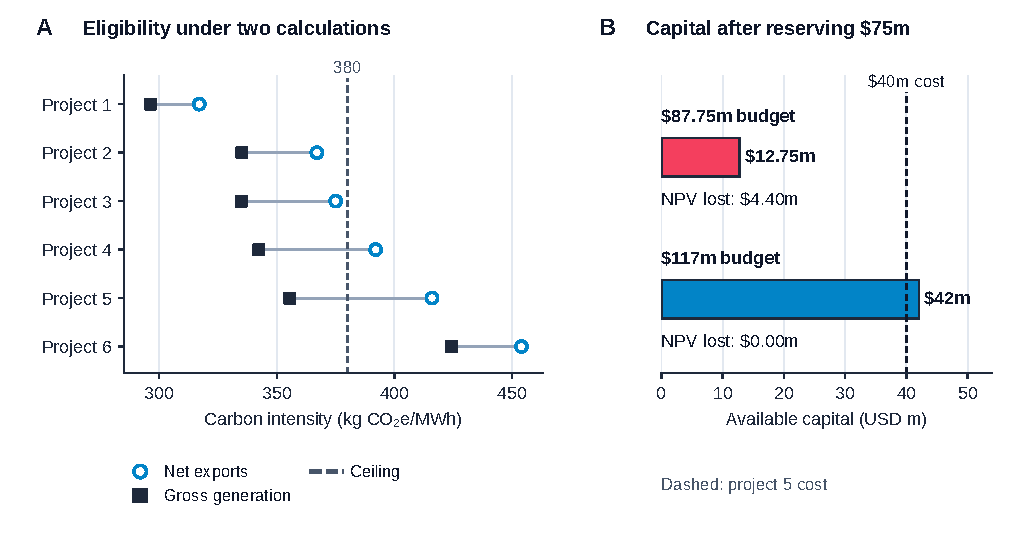
\includegraphics[width=\linewidth]{figures/project_example.pdf}
\caption{At one budget, admitting project~5 costs two other projects their funding. At the other, all three qualifying investments remain funded. (A) Each row shows a project in portfolio~1. Open circles use electricity exported to the grid and squares use all electricity generated. Scores at or below the dashed ceiling of 380~\unit\ qualify. (B) Reserving USD 75 million for projects~1--3 leaves the amounts shown by the bars. The dashed line marks project~5's USD 40 million cost. The losses are the net present value (NPV) of qualifying projects displaced.}\label{fig:project}

\end{figure*}
\fi



\subsection{What changes when projects cross the emissions ceiling?}
Both errors that lowered measured intensity increased total portfolio NPV on average while reducing the NPV of qualifying investments (Table~\ref{tab:money}). Across the 72 combinations of portfolio, budget and ceiling, the projects funded under the reference rule delivered a mean NPV of USD 14.97 million. The two errors changed 129 selections. In 55 of them the lender could add an ineligible project and keep its entire reference portfolio. These cases account for 31 changes under gross-output substitution and 24 under Scope~2 omission. In the other changed selections, the newly funded projects used capital needed by qualifying investments.
\ifdefined\readingcopy\ifdefined\readingcopy\begin{table*}[!t]\else\begin{table}[!ht]\fi\centering
\caption{How each carbon calculation changes funding relative to the specified formula. Each row covers 72 combinations of portfolio, ceiling and budget. The first two columns count decisions. The monetary columns report means in modeled USD millions. Qualified NPV includes only funded projects meeting the stated rule. Total NPV includes every funded project.}\label{tab:money}
\footnotesize\setlength{\tabcolsep}{4pt}
\begin{tabularx}{\linewidth}{@{}Xrrrrr@{}}\toprule
 & \shortstack[r]{Funded set\\changed} & \shortstack[r]{Positive\\shortfall} & \shortstack[r]{Ineligible\\capital} & \shortstack[r]{Qualified NPV\\shortfall} & \shortstack[r]{Change in\\total NPV}\\\midrule
Gross output & 63 & 32 & 48.833 & 1.974 & $+10.794$\\
Scope 2 omitted & 66 & 42 & 58.944 & 2.614 & $+13.316$\\
Net output understated & 69 & 69 & 0.000 & 13.237 & $-13.237$\\
Reference & 0 & 0 & 0.000 & 0.000 & 0.000\\\bottomrule
\end{tabularx}
\ifdefined\readingcopy\end{table*}\else\end{table}\fi
\fi



An error in the other direction removed projects from consideration entirely. Understating net exports raised measured intensity and wrongly excluded 57 of the 73 project--ceiling comparisons that qualified under the correct rule. All 69 resulting changes in funding reduced qualified NPV through exclusion. In the opposite direction, using gross generation wrongly admitted 44 of the 71 comparisons above the ceiling, and omitting Scope~2 admitted 53. Taken together, the 73 qualifying and 71 nonqualifying comparisons account for the 144 eligibility tests under each formula.

Eligibility alone did not determine whether funding changed. At least one project crossed the ceiling in 69 of the 72 financing decisions under gross substitution and in all 72 under each of the other errors. Allowing different formulas for different projects gave 1,848 combinations of eligibility patterns and financing decisions. Of these, 1,068 contained errors in both directions. Only 161 lost qualified value through both exclusion and ineligible spending (Equation~\eqref{eq:decompose}). A count of misclassified projects would miss that distinction.


\subsection{Which budgets and emissions ceilings change the funding decision?}
The original budget and ceiling settings lie in a particularly sensitive part of the policy range (Figure~\ref{fig:map}). Within the rectangle spanned by those settings, gross substitution changed the funded set over 92.4\% of the area on average across the eight portfolios. The corresponding shares were 98.3\% for Scope~2 omission and 97.8\% for net-output undercount. Across the full range of project scores and capital budgets, the three mean shares fell to 36.7\%, 42.8\% and 53.3\%. That range includes budgets too small to finance a project and ceilings at which the screens agree. Extending it beyond the lowest and highest calculated scores would add only unchanged allocations.
\ifdefined\readingcopy\begin{figure*}[!t]
\centering
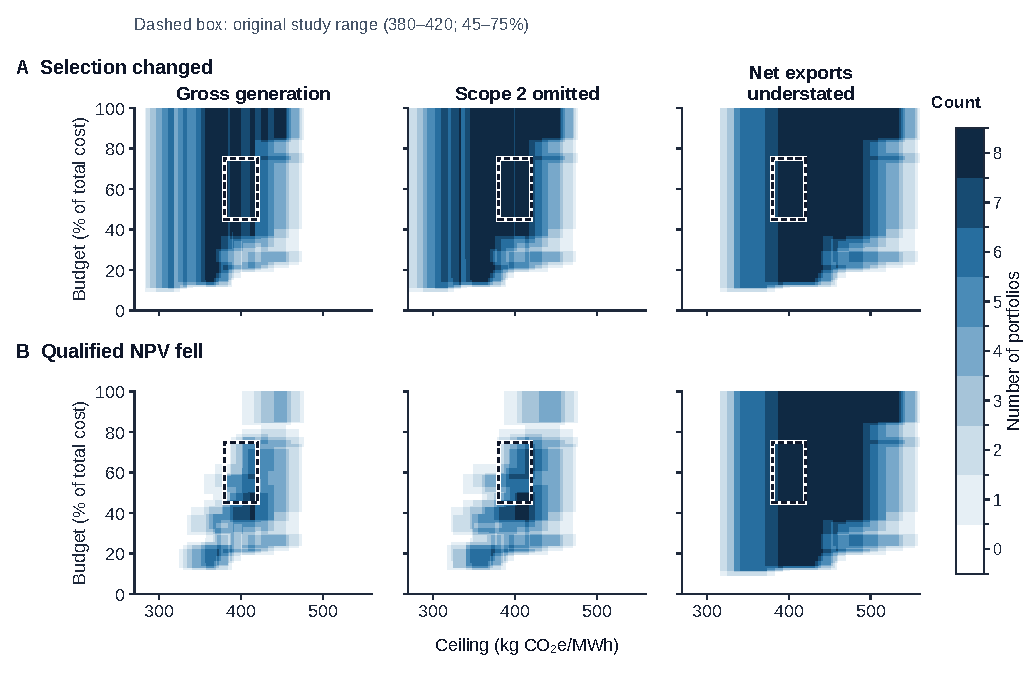
\includegraphics[width=\linewidth]{figures/policy_geometry.pdf}
\caption{Where a carbon calculation changes funding and where it reduces qualifying value. Each point represents an emissions ceiling and a budget. Within each column, the upper map (A) counts portfolios whose funded projects changed under the indicated error, and the lower map (B) counts those whose funded projects delivered less net present value under the stated eligibility rule. Both rows use the same scale from zero to eight portfolios. Boxes mark the original study range of 380--420~\unit\ and budgets of 45--75\% of the capital required for all six projects.}\label{fig:map}

\end{figure*}
\fi



Qualified NPV fell over a smaller share of the full rectangle under the two downward errors, averaging 12.1\% for gross substitution and 14.6\% for Scope~2 omission. Under net-output undercount, every change in selection reduced qualified NPV, giving 53.3\% for both outcomes.

A larger budget can finance more ineligible capital while displacing less qualified value. Between the original 45\% and 75\% budgets, gross substitution raised mean ineligible capital from USD 40.21 million to USD 54.13 million, while mean displacement fell from USD 3.51 million to USD 0.56 million. Extra capital could not restore projects excluded under net-output undercount. Its mean shortfall rose from USD 12.72 million to USD 13.62 million.

When the control projects started far from the ceiling, every one retained its eligibility. Writing $\widehat E_i$ for the intensity returned by an altered formula, the smallest margin $|E_i-\tau|-|\widehat E_i-E_i|$ across the three altered formulas was 29.55~\unit. This margin compares the distance to the ceiling with the magnitude of the calculation error: every error was too small to cross the ceiling. All 216 decisions under the altered formulas retained the same funded sets as their 72 corresponding reference decisions.

\subsection{Comparing upward and downward errors of equal size}
On the original projects, overstating intensity cost more qualified NPV on average than understating it by a matched factor (Table~\ref{tab:matched}). For each of the three changes implemented in the code, we also calculated what would happen if the error acted in the opposite direction by the same factor. We used the exact ratios to settle cases that fell on the ceiling. With the fixed multiplier, the two directions changed the funded set equally often. Raising measured intensity nevertheless cost almost five times as much qualified NPV on average.
\ifdefined\readingcopy\ifdefined\readingcopy\begin{table*}[!t]\else\begin{table}[!ht]\fi\centering
\caption{Effects of lowering and raising intensity by the same factor. Each direction uses 72 portfolio, ceiling and budget combinations. Changes count funded sets that differ from the reference. Shortfalls are mean losses in qualified NPV, in modeled USD millions.}\label{tab:matched}
\footnotesize\begin{tabularx}{.98\linewidth}{@{}Xrrrr@{}}\toprule
 & \multicolumn{2}{c}{Lower intensity $E_i/m_i$} & \multicolumn{2}{c}{Higher intensity $E_i m_i$}\\
\cmidrule(lr){2-3}\cmidrule(l){4-5}
Factor $m_i$ & Changes & Shortfall & Changes & Shortfall\\\midrule
Gross/net output $G_i/Q_i$ &63&1.974&66&11.506\\
Inverse Scope 1 share $1/(1-s_i)$ &66&2.614&66&12.685\\
Inverse output multiplier $1/0.85$ &69&2.720&69&13.237\\\bottomrule
\end{tabularx}
\ifdefined\readingcopy\end{table*}\else\end{table}\fi
\fi



Changing which costs and cash flows belong to which project can reverse the ranking for an individual funding decision (Table~\ref{tab:assignment}). Each scale yielded 51,840 comparisons of the two directions at a given portfolio, pairing, ceiling and budget. Under one reassignment in portfolio~5, with a ceiling of 420 and a 45\% budget, using gross generation in place of net exports directed USD 79 million to projects above the ceiling. It displaced the entire USD 12.11 million in reference qualified NPV. The matched upward error lost only USD 0.60 million in qualified NPV.
\ifdefined\readingcopy\ifdefined\readingcopy\begin{table*}[!t]\else\begin{table}[!ht]\fi\centering
\caption{Difference in qualified NPV loss between raising intensity and lowering it after financial profiles are reassigned. A local reversal is one portfolio, budget, ceiling and assignment in which the downward error costs more. The full-grid range gives the lowest and highest attainable mean difference over all eight portfolios and nine policy settings, in modeled USD millions. Positive values mean the upward error costs more. The last three columns hold the budget fixed and weight the ceilings equally. Endpoints are rounded to two decimals.}\label{tab:assignment}
\footnotesize\setlength{\tabcolsep}{4pt}
\begin{tabularx}{\linewidth}{@{}Xrrrrr@{}}\toprule
 &\shortstack[r]{Local reversals\\of 51,840} & \shortstack[r]{Full grid\\sharp range} &\multicolumn{3}{c}{Lowest mean at fixed budget}\\
\cmidrule(l){4-6}
Factor & & & 45\% & 60\% & 75\%\\\midrule
Gross/net output & 2,098 & [1.60, 18.90] & $-1.83$ & $1.54$ & $3.84$\\
Inverse Scope 1 share & 1,748 & [1.69, 21.03] & $-1.90$ & $1.63$ & $4.27$\\
Inverse output multiplier & 740 & [1.67, 21.77] & $-1.77$ & $1.67$ & $4.77$\\\bottomrule
\end{tabularx}
\ifdefined\readingcopy\end{table*}\else\end{table}\fi
\fi



Table~\ref{tab:assignment} shows that the smallest attainable average difference (the lower bound) is positive at all three error scales when all nine budget--ceiling settings are included, and negative when only the 45\% budget is used. Thus, with equal weight on the eight portfolios, three ceilings and three budgets, overstatement causes greater mean loss under every joint assignment. At the 45\% budget, a single joint assignment gave upward-minus-downward mean differences of USD $-1.28$, $-1.90$ and $-0.90$ million for the gross-to-net, inverse Scope~1 and fixed scales, respectively, averaging equally across ceilings. At the 60\% and 75\% budgets, the lower bound remained positive for every scale. The directional ranking therefore depends on the budget.

\subsection{How many checks identify the funded projects?}
When all six projects used the same formula, checking whether one project qualified could settle the funding decision for another. In portfolio~1 at the 380 ceiling and 45\% budget, project~4 had negative NPV and could never win funding. Yet once project~2 qualified, checking project~4 distinguished the correct formula from the two that lowered measured intensity. A check on a project that would remain unfunded could therefore reveal which other projects qualified.

At most two checks identified the funded set at each of the 72 settings with a shared formula. Moving from the strictest formula to the most permissive only added eligible projects. Checking a project whose status differed across the possible formulas could therefore rule out several possibilities at once.

When projects could use different formulas, more eligibility checks were needed. In the same example, the answer for project~4 told the reviewer nothing about project~5. The reviewer could nevertheless stop once two selections agreed. These were the best portfolio using only projects certain to qualify and the best using every project that might qualify. That same portfolio wins for every intermediate set. If the two selections differ, either remains possible, and another check is needed. This raised the worst-case requirement to five checks. An adaptive strategy selects each check after seeing the previous answer; a fixed strategy chooses the complete list beforehand. Adding the separate worst-case counts for all 72 decisions, the adaptive strategy required 135 checks under a shared formula, compared with 155 for the best fixed lists. With project-specific formulas, both strategies took 285 checks. Resolving every uncertain project's status would have taken 330. The advantage of choosing checks adaptively therefore depends on whether projects share a formula.

\subsection{What the source files reveal about a calculation error}
LEAP and the simpler annotation-reading program recovered the same documentation fields across the 192 main files. LEAP linked the indicator name and written formula to line~1, where the KPI record begins, and retained the nearby code that returns the calculated intensity at line~10. The formula declaration was on line~4. Across the four file templates, both programs recovered the same file names, standardized indicator names, formulas and lines identifying the start of each KPI record. This establishes the extraction result for the annotated files used in the study.

Comparing the written and implemented operations identified all 144 deliberately altered files. Running the programs on the project inputs and comparing their outputs with the expected values identified the same 144. The additional cases in Supplement~S1 show where the two checks diverge. Reordering the two terms in the numerator triggered a structural mismatch while preserving the numerical value. In another case, an outdated written formula and its matching implementation passed the structural comparison while returning 36 instead of the reference-rule intensity of 40 on the constructed inputs. To assess the financial consequence, the reviewer must follow that answer into the funding decision.

\section{Discussion}
A carbon calculation error can cost qualifying investment value in two ways: excluding projects can lower the best attainable qualifying NPV, and admitting ineligible projects can divert capital needed by qualifying investments. Equation~\eqref{eq:slack} identifies exactly when the second mechanism begins. Ineligible spending must exceed the money left after reserving the least expensive optimal combination of projects that pass both calculations. The amount of value displaced then depends on the investments that the remaining capital can finance.

The most consequential distinction for an investment committee is between spending outside the mandate and the value of qualifying opportunities forgone. An ineligible project with positive NPV can raise total portfolio NPV while reducing qualified NPV. When an error also excludes qualifying projects, Equation~\eqref{eq:decompose} values the exclusions at the full budget before measuring displacement among projects still eligible under both calculations. This provides a financial account of the consequences under a fixed emissions ceiling, distinct from assigning monetary weights to environmental outcomes \citep{schoenmaker}.

The findings extend research on the relationship between carbon measurement and investment selection. \citet{anquetin} compare investment choices under different emissions measures; \citet{gurvich2021} and \citet{bajic2023} identify how erroneous or inconsistent carbon information can affect screening and rankings. We hold the approved rule fixed and trace an error through the subsequent funding decision. Equations~\eqref{eq:loss} and \eqref{eq:decompose} value the resulting eligibility errors under capital rationing, separating losses from excluding qualifying projects and financing falsely admitted ones. The results show why changed allocations are an insufficient measure of financial loss: a lender may add an ineligible project and still fund the complete reference portfolio.

The effects of an error depend on the eligibility boundary and the available capital. The policy maps (Figure~\ref{fig:map}) show where different emissions ceilings and budgets change funding, and the control projects retain their eligibility when the errors do not cross the ceiling. When the same factor raises or lowers intensity, overstatement causes greater average losses across the equally weighted policy settings under every joint financial assignment. The tightest budget allows the ranking to reverse. The error direction and magnitude must therefore be interpreted alongside the investment decision.

\subsection{Implications for environmental investment governance}
For an investment committee, the result provides a way to connect carbon-accounting governance to capital approval. \citet{ruan2026} identify the organizational arrangements that embed emissions accounting; our displacement condition (Equation~\eqref{eq:slack}) makes the financial consequence of a calculation error measurable for a defined investment choice. An assurance record for each funding decision should link the approved rule, its implementation, the competing projects and their budget. This applies the measurement and accountability concerns discussed by \citet{tian2026} to the specific decision through which an environmental strategy allocates capital.

The committee can then use three quantities to assess the decision: capital committed outside the approved rule, qualified NPV lost by excluding eligible projects, and qualified NPV displaced by financing ineligible projects. The first measures the amount spent outside the mandate; the other two measure the opportunities forgone (Equation~\eqref{eq:decompose}). Presenting them together reveals a financial consequence that an increase in total portfolio NPV would obscure (Table~\ref{tab:money}).

The verification analysis also identifies when sustainability assurance teams can focus their checks on the information needed to resolve a funding decision. When projects share a formula, checking one informative project may resolve several eligibility questions. When formulas vary independently, more project-level checks may be needed. A proposed governance process would start with the approved emissions boundary and denominator, trace the implemented formula and its version, re-evaluate eligibility, and retain the before-and-after allocations and their financial loss. The record would connect sustainability assurance to capital approval, complementing firm-level research on audit quality and reported emissions intensity \citep{ibrahim2026}.

\subsection{Scope and limitations}
The threshold applies to any finite set of indivisible projects with one budget, positive additive costs, additive values, and the option to leave funds unspent. If one project changes another's cash flows, or a financing agreement restricts which projects can be financed together, the remaining capital alone may no longer determine displacement.

The 48 main projects come from one constructed design. Reassigning costs and cash flows preserves the financial profiles and the relationships among emissions inputs. The policy-map shares describe the specified range of ceilings and budgets for these projects. Estimating how frequently errors occur, their typical financial consequences or their effects on actual emissions would require project and lending records, including the policies lenders use.

Estimating the financial effect of a real calculation error requires separating it from other changes in measurement. At Copiulemu, methane revisions changed both a spreadsheet column and the assumed flare efficiency, the proportion of methane destroyed by burning \citep[pp.~9--11, 14]{sgs}. Measuring the column's contribution would require holding flare efficiency and the other inputs fixed.

Valuing the alternatives requires financing records. The Vasilikos appraisal reports an emissions estimate and gives no indication of a coding defect. The loan register records the amount signed \citep{eibscore,eibloan}. Applying our screen would require knowing which emissions the bank counted and whether it used net exports. Measuring displacement would also require the competing proposals, their costs and cash flows, the budget and eligibility under both calculations.

The verification model assumes a known list of possible formulas and accurate, equally costly answers. With a shared formula, checking an unfunded project can reveal which others qualify. With project-specific formulas, it settles only that project's status. Partial sharing or unequal costs could change which check is worth doing first. Estimating analyst time would require measuring the work each answer takes.

\section{Conclusions}
The opportunity cost of a carbon calculation error is the shortfall in qualified NPV relative to the best portfolio the approved rule allows. It can be measured from the competing project list and capital budget. First, value projects wrongly excluded by comparing the best qualifying portfolios before and after exclusion. Then value the opportunities displaced by financing falsely admitted projects. Among projects passing both calculations, the least expensive combination achieving the highest NPV determines how much capital can be spent on ineligible projects without displacing qualifying value. The same error can therefore produce different losses at different budgets. For environmental investment governance, the result makes it possible to assess the financial consequence of an erroneous eligibility decision before committing capital.

\section*{Supporting information and data availability}
Supplement S1 contains the constructed project registers, annotated source files, original implementation and control results, and reproducibility scripts. It includes comparisons for each funding decision, the exclusion and displacement components, sensitivity to error direction and financial reassignment, the full policy map, verification-count calculations and source-inspection cases. \ifdefined\readingcopy
The data and replication code are publicly available in Harvard Dataverse (Version 1.0), \href{https://doi.org/10.7910/DVN/ZSXX0E}{doi:10.7910/DVN/ZSXX0E}. The associated research repository is \href{https://github.com/Meshaal-Mouawad/paper-10-green-capital-budgeting}{GitHub (paper-10-green-capital-budgeting)}.
\else
The replication repository identifiers are provided separately with the author information for double-anonymous review.
\fi
